% 第 8 章 The Cordoba Multiplier Theorem (原书第 126-146 页)
\chapter{C\'ordoba 乘子定理}
\label{chap:8}

\section{殆正交性}
\label{sec:8.1}
\index{殆正交性!与曲率 (almost orthogonality and curvature)}

奇性的标准模型提示, 我们需要对 $\phi_{\delta}(\xi)=\phi\bigl(\delta^{-1}(|\xi|-1)\bigr)$ 及其乘子性质给出一个好的估计. 对于短论~\ref*{ess:7.3} 中的反例函数, $T_{\delta}f_j=T_0f_j$, 于是我们预计 ${}_4\|T_{\delta}\|\geq C|\log\delta|^{\frac{1}{4}}$. 若事实上这个下界接近真实的算子范数, 则标准模型提示 $\mu_{\lambda}=\sum 2^{-\lambda j}\phi_{2^{-j}}$, 于是
\[
{}_{4}\|T_{\lambda}\|\leq\sum 2^{-\lambda j}\,{}_4\|T_{2^{-j}}\|\leq C\sum 2^{-\lambda j}\,j^{\frac{1}{4}}<\infty
\]
当 $\lambda>0$ 时成立. 这将证明所有 $T_\lambda$ 的 $L^4$ 有界性, 而对偶与内插便会像图~\ref{fig:12} 所勾画的那样, 在其余各处证明最优结果.

~\ref*{ess:7.3} 中的计算提示, $\phi_{\delta}$ 应当被分解成大小为 $\delta\times\delta^{\frac{1}{2}}$ 的小矩形; 在控制了每一个的范数之后, 我们还须证明 Meyer 引理的某种逆命题, 把各个矩形的作用分离开来. 于是我们从建立正交性结果开始.

\begin{figure}[htbp]
\centering
\begin{tikzpicture}[scale=0.9]
  % 阴影区域 (斜线填充)
  \fill[pattern=north west lines, pattern color=black!70]
    (0,2) -- (1.25,0) -- (3.75,0) -- (5,2) -- (5,4) -- (0,4) -- cycle;
  \draw (0,0) rectangle (5,4);
  \draw[dashed] (0,2) -- (1.25,0);
  \draw[dashed] (3.75,0) -- (5,2);
  \draw (0,2) circle (2.4pt);
  \draw (5,2) circle (2.4pt);
  \draw (1.25,0) circle (2.4pt);
  \draw (3.75,0) circle (2.4pt);
  \fill (1.8,0) circle (2.2pt);
  \fill (3.2,0) circle (2.2pt);
  \node[right] at (5.1,2.6) {$\alpha=\frac{1}{2}$};
  \node[below] at (1.25,-0.15) {$\frac{1}{p}=\frac{1}{4}$};
  \node[below] at (3.75,-0.15) {$\frac{1}{p}=\frac{3}{4}$};
\end{tikzpicture}
\caption{圆周乘子的多尺度矩形分解}
\label{fig:12}
\end{figure}

\begin{theorem}\label{thm:8.1}
设 $I_j$ 是等长、内部互不相交且并集为整个 $\mathbb{R}$ 的区间. 设 $P_j$ 是以 $\chi_{I_j}$ 为乘子的乘子算子. 若 $2\leq p<\infty$, 则
\[
\Bigl\|\Bigl(\sum_{j}|P_{j}f|^{2}\Bigr)^{\frac{1}{2}}\Bigr\|_{p}\leq C\|f\|_{p}.
\]
\end{theorem}

\begin{proof}
区间网格可以平移为形如 $I_{j}=(ja,(j+1)a)$ 的区间; 这只是把 $f$ 改变了一个等距算子. 再伸缩得 $(j,j+1)$, 又经平移得 $\bigl(j-\frac{1}{2},j+\frac{1}{2}\bigr)$. 我们得出: 定理中的范数与区间的大小无关.

在证明 Littlewood--Paley 不等式时, 我们需要: a) 结果的一个光滑版本; b) 为证明 a) 所需的一个乘子定理; c) 一个正交化步骤. 为构造乘子结果, 设 $\psi$ 是光滑函数, 在 $I_0$ 上 $\psi=1$, 在 $\tilde{I}_0$ 之外 $\psi=0$. 设 $T_j$ 是对应于 $\psi(\xi-j)$ 的乘子算子; 注意 $P_jf=P_jT_jf$. 由于 H\"ormander--Mikhlin 定理不适用于 $\sum T_j$, 我们需要一个新窍门, 而它将同时解决我们对正交性的需求. 令
\[
\mu(\xi)=\sum_j e^{2\pi ij\theta}\,\psi(\xi-j);\qquad k=\check{\mu}.
\]
则
\[
\int_{I_{0}}\bigl|k\star f(x)\bigr|^{2}\,d\theta
=\int_{I_{0}}\Bigl|\sum_j e^{2\pi ij\theta}\,T_{j}f(x)\Bigr|^{2}\,d\theta
=\sum_j\bigl|T_{j}f(x)\bigr|^{2},
\]
最后一步用了 $I_0$ 上的 Plancherel 定理. 但问题关乎与 $k$ 作卷积的 $L^{p}$ 行为; 为此我们使用 Poisson 求和公式 (参见 Stein 与 Weiss~\cite{steinweiss} 第~7 章第~2 节).

若 $f\in L^1(\mathbb{R})$, $\theta\in I_0$, 则
\[
\sum_j\hat{f}(j)\,e^{2\pi ij\theta}=\sum_j f(\theta+j);
\]
这里 $\hat{f}(j)=\int e^{-2\pi ijy}f(y)\,dy$. 在我们的情形, 需要 $\hat{f}(j)=\psi(\xi-j)$, 于是令
\[
f(x)=\int e^{2\pi iyx}\,\psi(\xi-y)\,dy=e^{2\pi ix\xi}\,\hat{\psi}(x).
\]
由于 $\psi\in\mathcal{S}$, 故 $f\in L^1$. 则
\[
\sum_j\psi(\xi-j)\,e^{2\pi ij\theta}=\sum_j e^{2\pi i(j+\theta)\xi}\,\hat{\psi}(\theta+j),
\]
且
\[
k(x)=\sum_j\bigl[e^{2\pi i(j+\theta)\xi}\bigr]^{\vee}(x)\,\hat{\psi}(\theta+j)
=\sum_j\delta_{j+\theta}(x)\,\hat{\psi}(j+\theta).
\]
现在, 与 $k$ 作卷积的 $L^{p}$ 算子范数由 $k$ 的全变差范数给出:
\[
\|k\|\leq\sum_j\bigl|\hat{\psi}(j+\theta)\bigr|\,\|\delta_{j+\theta}\|
\leq\sum_j\bigl|\hat{\psi}(j+\theta)\bigr|
\leq C\sum_j\bigl((j+\theta)^{2}+1\bigr)^{-1}\leq C.
\]
这控制了乘子范数; 最后我们需要从 $L^{2}$ 过渡到 $L^{p}$; 我们将使用 H\"older 不等式而非独立性. 则
\[
\int\Bigl(\sum|P_{j}f|^{2}\Bigr)^{\frac{p}{2}}
=\int\Bigl(\sum|P_{j}T_{j}f|^{2}\Bigr)^{\frac{p}{2}}
\leq C\int\Bigl(\sum|T_{j}f|^{2}\Bigr)^{\frac{p}{2}},
\]
最后一步用了命题~\ref{prop:4.12}. 而后者又等于
\begin{align*}
C\int\left(\int_{I_{0}}|k\star f|^{2}\,d\theta\right)^{\frac{p}{2}}dx
&=C\int\bigl(\|k\star f\|_{2,\theta}\bigr)^{p}\,dx
\leq\int\bigl(\|k\star f\|_{p,\theta}\bigr)^{p}\,dx \\
&=C\iint_{I_{0}}|k\star f|^{p}\,d\theta\,dx
=C\int_{I_{0}}\int_{\mathbb{R}}|k\star f|^{p}\,dx\,d\theta \\
&\leq C\|k\|\int_{I_{0}}\int|f|^{p}\,dx\,d\theta=C\|f\|_{p}^{p}. \qedhere
\end{align*}
\end{proof}

\begin{corollary}\label{cor:8.2}
设 $B_j=\{(\xi_1,\xi_2) \mid \xi_2\in I_j\}$, 并设 $S_j$ 是以 $\chi_{B_j}$ 为乘子的算子. 则对 $2\leq p<\infty$,
\[
\Bigl\|\Bigl(\sum|S_{j}f|^{2}\Bigr)^{\frac{1}{2}}\Bigr\|_{p}\leq C\|f\|_{p}.
\]
\end{corollary}

\textbf{证明概要}: 由于 $S_j$ 在 $\xi_1$ 方向上如同恒等算子, 该结果是定理~\ref{thm:8.1} 与恒等算子的乘积. 形式上, 对每个 $x_1$ 定义函数 $g(x_2)=f(x_1,x_2)$, 并注意对几乎所有的 $x_1$, $g\in L^1$ 且 $(S_jf)(x_1,x_2)=(P_jg)(x_2)$. 等等.

\begin{remark}\label{rem:8.3}
诸 $I_j$ 的规则分布对定理~\ref{thm:8.1} 的证明并非本质; 我们真正用到的只是 $\psi_j(\xi)=\psi(\xi-j)$ 以及 $\chi_{I_j}\psi_j=\chi_{I_j}$. 这意味着诸 $I_j$ 可以做一些手脚而定理仍然成立. 当然我们可以每隔一个丢掉一个, 从而假设 $\operatorname{distance}(I_j,I_{j+1})\geq c>0$. 但我们还必须要求诸 $I_j$ 的长度与它们的间距以及彼此之间可比:
\[
c_{1}\leq d(I_{j},I_{j+1})\leq c_{2},
\qquad
c_{1}\leq|I_{j}|\leq c_{2}.
\]
我们心中其实已有一个应用: 令
\[
C_{j}=\bigl\{(r,\theta) \,\big|\, j\leq\delta^{-\frac{1}{2}}\theta\leq j+1\bigr\},
\]
并设 $I_{j}$ 是 $C_{j}$ 在 $\xi_{2}$ 轴上的投影. 则
\[
|I_{j}|\approx\delta^{\frac{1}{2}}\,\Bigl|\sin\Bigl(\frac{2\pi j}{\delta^{\frac{1}{2}}}\Bigr)\Bigr|,
\]
于是诸 $I_j$ 的长度不可比. 若把诸 $I_j$ 分成四组, 每组落在围绕 $\frac{\pi}{4}$ 系直线的某个锥形中, 并对每个锥中的区间用单独的平方函数处理, 那么在每个锥内我们就能保证大小可比.
\end{remark}

\essayhead{ess:8.4}{殆正交性与曲率}

不幸的是, 推论~\ref{cor:8.2} 还不够好; 为得到乘子定理, 我们需要形如
\[
\|T_{\delta}f\|_{4}\leq\Bigl\|\Bigl(\sum|S_{j}T_{\delta}f|^{2}\Bigr)^{\frac{1}{2}}\Bigr\|_{4}
\leq\Bigl\|\Bigl(\sum|P_{j}f|^{2}\Bigr)^{\frac{1}{2}}\Bigr\|_{4}
\]
的不等式; 推论~\ref{cor:8.2} 只允许我们从 $\sum|P_jf|^2$ 走到 $|f|$, 所以我们还需要一些正交性. 为看清需要什么, 设 $C_j$ 表示锥
\[
\{(r,\theta) \mid j\leq\delta^{-\frac{1}{2}}\theta\leq j+1\},
\]
并设 $\mu_j=\chi_{C_j}\phi_\delta$. 如上所述, 我们只处理落在锥 $0\leq\theta\leq\frac{\pi}{4}$ 中的 $C_j$. 若 $T_j$ 是对应于 $\mu_j$ 的算子, 令 $T^0=\sum T_j$. 设 $I_j$ 表示诸 $\mu_j$ 的支集在 $\xi_2$ 轴上的投影, 并设 $S_j$ 是以 $\chi_{I_j}(\xi_2)$ 为乘子的算子. 则 $S_jT_j=T_j$, 且估计
\[
\Bigl\|\sum T_{j}f\Bigr\|_{4}=\Bigl\|\Bigl(\sum|T_{j}f|^{2}\Bigr)^{\frac{1}{2}}\Bigr\|_{4}
\]
将蕴含
\[
\|T^{0}f\|_{4}=\Bigl\|\sum T_{j}f\Bigr\|_{4}
\leq C\Bigl\|\Bigl(\sum|T_{j}f|^{2}\Bigr)^{\frac{1}{2}}\Bigr\|_{4}
=\Bigl\|\Bigl(\sum|S_{j}T_{j}f|^{2}\Bigr)^{\frac{1}{2}}\Bigr\|_{4}.
\]
我们希望把它控制为
\[
C\Bigl\|\Bigl(\sum|S_{j}f|^{2}\Bigr)^{\frac{1}{2}}\Bigr\|_{4},
\]
而后者可以用~\ref*{cor:8.2} 处理. 于是我们需要两个不等式:
\begin{align*}
\Bigl\|\sum T_{j}f\Bigr\|_{4}&\leq C\Bigl\|\Bigl(\sum|T_{j}f|^{2}\Bigr)^{\frac{1}{2}}\Bigr\|_{4}, \\
\Bigl\|\Bigl(\sum|S_{j}T_{j}f|^{2}\Bigr)^{\frac{1}{2}}\Bigr\|_{4}
&\leq C\Bigl\|\Bigl(\sum|S_{j}f|^{2}\Bigr)^{\frac{1}{2}}\Bigr\|_{4}.
\end{align*}
为分析第一个, 我们取四次幂: 我们需要
\[
\int\Bigl|\sum T_{j}f\Bigr|^{4}\leq C\int\Bigl(\sum|T_{j}f|^{2}\Bigr)^{2},
\]
即
\[
\int\Bigl|\Bigl(\sum T_{j}f\Bigr)\Bigl(\sum T_{k}f\Bigr)\Bigr|^{2}
\leq C\int\sum|T_{j}f|^{2}\,|T_{k}f|^{2}.
\]
先把积分搁在一边; 我们是在要求
\[
\Bigl(\sum|a_{j}|\Bigr)^{2}\leq C\sum|a_{j}|^{2}.
\]
这非常奇特; 所有真实的不等式, 比如 $(a+b)^2\geq a^2+b^2$, 方向都相反. 当然 $(a+b)^2\leq 2(a^2+b^2)$ 是对的, 但平方里项数越多它越不成立. 因此积分是关键的: 我们最好指望, 若 $x$ 落在某个 $T_jfT_kf$ 的支集之中, 它就不落在其他的支集之中. 简言之, 我们希望诸 $T_jfT_kf$ 在 $L^2$ 上正交.

当然, 这是 $L^{2}$, 而正交性在 Fourier 变换一侧应当有意义:
\begin{align*}
\|T^{0}f\|_{4}^{4}
&=\int\Bigl|\sum_{j,k}\bigl(\mu_{j}\hat{f}\bigr)\star\bigl(\mu_{k}\hat{f}\bigr)\Bigr|^{2}.
\end{align*}
若 $A_{jk}$ 表示
\[
\bigl(\mu_{j}\hat{f}\bigr)\star\bigl(\mu_{k}\hat{f}\bigr)
\]
的支集, 我们将证明: 对所有的 $\xi$, $\sum\chi_{A_{jk}}(\xi)\leq 9$, 即没有一个 $\xi$ 落在多于 $9$ 个的 $A_{jk}$ 之中. 这是完全不相交的替代品, 蕴含正交性. 它同样好用, 因为
\begin{align*}
\Bigl|\sum\bigl(\mu_{j}\hat{f}\bigr)\star\bigl(\mu_{k}\hat{f}\bigr)\Bigr|
&=\Bigl|\sum\bigl(\mu_{j}\hat{f}\bigr)\star\bigl(\mu_{k}\hat{f}\bigr)\chi_{A_{jk}}\Bigr| \\
&\leq\Bigl(\sum|\chi_{A_{jk}}|^{2}\Bigr)^{\frac{1}{2}}
\Bigl(\sum\bigl|\mu_{j}\hat{f}\star\mu_{k}\hat{f}\bigr|^{2}\Bigr)^{\frac{1}{2}} \\
&\leq 3\Bigl(\sum\bigl|\mu_{j}\hat{f}\star\mu_{k}\hat{f}\bigr|^{2}\Bigr)^{\frac{1}{2}}.
\end{align*}
平方并积分,
\begin{align*}
\|T^{0}f\|_{4}^{4}
&=\int\Bigl|\sum\bigl(\mu_{j}\hat{f}\bigr)\star\bigl(\mu_{k}\hat{f}\bigr)\Bigr|^{2}
\leq 9\int\sum\bigl|\bigl(\mu_{j}\hat{f}\bigr)\star\bigl(\mu_{k}\hat{f}\bigr)\bigr|^{2} \\
&=9\int\sum|T_{j}f|^{2}\,|T_{k}f|^{2}
=9\int\Bigl(\sum|T_{j}f|^{2}\Bigr)^{2}
=9\Bigl\|\Bigl(\sum|T_{j}f|^{2}\Bigr)^{\frac{1}{2}}\Bigr\|_{4}^{4},
\end{align*}
于是分析的第一部分完成. 为证 $\sum\chi_{A_{jk}}\leq 9$, 我们注意到
\[
A_{jk}=\operatorname{support}\,(\check{\mu}_{j}\star\check{\mu}_{k})
=\operatorname{support}\,\check{\mu}_{j}+\operatorname{support}\,\check{\mu}_{k}.
\]
我们面前的任务是一个几何任务: 我们必须分析诸 $A_{jk}$ 的交, 即环面的扇区之和. 实际的几何图景很复杂; 图~\ref{fig:13} 画的是若诸 $\mu_j$ 支在一个圆上而非环形区域上时图景的样子; 在图~\ref{fig:14} 中我们画出一个实际的 $A_{jk}$. 为证明不相交性, 诸 $A_{jk}$ 必须在角向与径向上分开. 若 $v_j$ 是 $\mu_j$ 支集中心处的单位向量, 则 $A_{jk}$ 是关于方向 $v_j+v_k$ 对称的集合. 这样的方向对至多有 $C\delta^{-\frac{1}{2}}$ 个; 沿着其中每一个, $A_{jk}$ 包含在半径为 $2\delta^{\frac{1}{2}}$ 的球中. 我们取球的中心为 $v_j+v_k$. 由于这些向量等距分布, 围绕 $v_j+v_k$ 的一个锥便把诸 $A_{jk}$ 彼此隔开; 我们可以得出结论: $A_{jk}\cap A_{jk'}\neq\varnothing$ 蕴含 $|(j+k)-(j'+k')|<2$. 这就完成了角向的隔离.

对于径向, 注意 $A_{jk}$ 的中心在
\[
\Bigl(1-\frac{\delta}{2}\Bigr)\bigl(\cos\theta_{j}+\cos\theta_{k},\ \sin\theta_{j}+\sin\theta_{k}\bigr);
\]
精确到 $\delta$ 的量级, $\theta_j=j\delta^{\frac{1}{2}}$. 诸 $A_{jk}$ 的中心之间的距离因此是向量
\[
\Bigl(1-\frac{\delta}{2}\Bigr)\bigl(\cos\theta_{j}-\cos\theta_{j-1}+\cos\theta_{k}-\cos\theta_{k+1},\ \ldots\bigr)
\]
的长度, 即
\begin{align*}
2\Bigl(1-\frac{\delta}{2}\Bigr)\Bigl(\sin\Bigl(\frac{\theta_{j}+\theta_{j-1}}{2}\Bigr)\sin\Bigl(\frac{\theta_{j}-\theta_{j-1}}{2}\Bigr)&\\
+\sin\Bigl(\frac{\theta_{k}+\theta_{k+1}}{2}\Bigr)&\sin\Bigl(\frac{\theta_{k}-\theta_{k+1}}{2}\Bigr),\ \cdots\Bigr).
\end{align*}
由于精确到 $\delta$ 的量级有 $\theta_j-\theta_{j-1}=\delta^{\frac{1}{2}}$, 诸中心的间距为 $\delta^{\frac{1}{2}}$, 精确到 $\delta$ 的量级.

因此, 沿方向 $v_j+v_k$ 的诸集合 $A_{jk}$ 构成 $\delta^{-\frac{1}{2}}$ 个集合, 每个包含在半径为 $2\delta^{\frac{1}{2}}$ 的球中, 其中心沿 $v_j+v_k$ 方向的一条直线均匀分布. 于是, 沿一条直线没有一个球能与多于两个其他的球重叠, 而在相邻的直线上至多与三个重叠. 这样, 平面上的任何一点至多属于 $9$ 个的 $A_{jk}$.

现在我们需要理解不等式
\[
\Bigl\|\Bigl(\sum|S_{j}T_{j}f|^{2}\Bigr)^{\frac{1}{2}}\Bigr\|_{4}
\leq\Bigl\|\Bigl(\sum|S_{j}f|^{2}\Bigr)^{\frac{1}{2}}\Bigr\|_{4}.
\]
若回忆 Marcinkiewicz 定理, 即定理~\ref{thm:4.14} 的证明, 我们看到需要形如
\[
\int|S_{j}T_{j}f|^{2}\,g\leq\int|S_{j}f|^{2}\,g^{\star}
\]
的不等式, 其中 $g^{\star}$ 是某种极大函数. 按照第~\ref{chap:7} 章的思路, $S_jT_jf$ 在 $v_j$ 方向上如同一个 Hilbert 变换. 若 $M_j$ 是该方向上的一维极大函数, 我们从第~\ref{chap:3}、\ref{chap:4} 章预计
\[
\int|S_{j}T_{j}f|^{2}\,g\leq\int|S_{j}f|^{2}\,\bigl[M_{j}(g^{s})\bigr]^{\frac{1}{s}},
\]
从而
\begin{align*}
\int\sum|S_{j}T_{j}f|^{2}\,g
&\leq\int\sum|S_{j}f|^{2}\,\sup_{j}\bigl[M_{j}(g^{s})\bigr]^{\frac{1}{s}} \\
&\leq\Bigl\|\Bigl(\sum|S_{j}f|^{2}\Bigr)^{\frac{1}{2}}\Bigr\|_{4}^{2}\,
\Bigl\|\sup_{j}\bigl[M_{j}(g^{s})\bigr]^{\frac{1}{s}}\Bigr\|_{2};
\end{align*}
剩下的唯一问题是控制极大函数. 这一做法确实成功, 但 $S_jT_j$ 实际上对应于 $\mu_j$, 它不如 Hilbert 变换奇异; 若把这一点考虑进去, 极大函数将更容易控制. 直观上, $\mu_j$ 是大小为 $\delta\times\delta^{\frac{1}{2}}$ 的矩形的特征函数; 因此 $T_j$ 的作用应当如同在一个具有对偶大小 $\delta^{-1}\times\delta^{-\frac{1}{2}}$ 的矩形上作平均. 这正是我们需要控制的那类极大函数.

\begin{figure}[htbp]
\centering
\begin{minipage}[b]{0.42\textwidth}
\centering
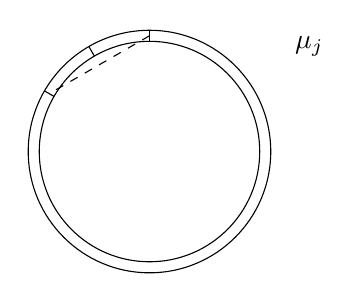
\begin{tikzpicture}[scale=0.7]
  % 图 13: 圆与扇区
  \draw (0,0) circle (2.2);
  \draw (0,0) circle (2.0);
  \foreach \a in {90,120,150} {
    \draw (\a:2.0) -- (\a:2.2);
  }
  \draw[dashed] (90:2.1) -- (150:2.1);
  \node at (2.9,1.9) {$\mu_j$};
\end{tikzpicture}
\caption{圆环支集的弧段扇区划分}
\label{fig:13}
\end{minipage}\hfill
\begin{minipage}[b]{0.42\textwidth}
\centering
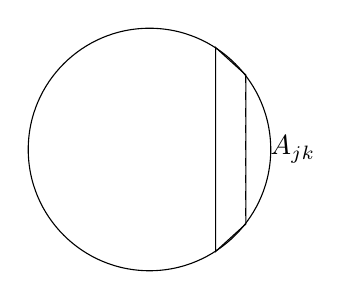
\begin{tikzpicture}[scale=0.7]
  % 图 14: 单个 A_jk
  \draw (0,0) circle (2.2);
  \draw[dashed] (1.2,1.85) -- (1.2,-1.85);
  \draw[dashed] (1.75,1.35) -- (1.75,-1.35);
  \draw (1.2,1.85) -- (1.75,1.35) -- (1.75,-1.35) -- (1.2,-1.85) -- cycle;
  \node at (2.6,0) {$A_{jk}$};
\end{tikzpicture}
\caption{相交区域 $A_{jk}$ 的截口形态}
\label{fig:14}
\end{minipage}
\end{figure}

\section{C\'ordoba 极大函数}
\label{sec:8.2}

\begin{definition}\label{def:8.5}
\index{Cordoba 极大函数 (C'ordoba maximal function)|emph}
取定 $N>1$, $a>0$. 设
\[
\mathcal{B}=\{R \mid R\ \text{是尺寸为}\ a\times aN\ \text{的矩形}\}.
\]
C\'ordoba 极大函数 $\mathcal{C}$ 定义为
\[
\mathcal{C}f(x)=\sup\frac{1}{|R|}\int_{R}|f(y)|\,dy,
\]
其中上确界取遍 $\mathcal{B}$ 中所有包含 $x$ 的矩形.
\end{definition}

\begin{theorem}\label{thm:8.6}
\[
\|\mathcal{C}f\|_{2}\leq C\,(\log 6N)^{\frac{1}{2}}\,\|f\|_{2}.
\]
\end{theorem}

\begin{proof}
诸如 $\bigl\|\sum\chi_{R_j}\bigr\|_2^2=\sum_{j,k}|R_j\cap R_k|$ 的量可以像第~\ref{chap:7} 章那样控制, 这便产生我们需要的对数项. 不幸的是, 构成 $\mathcal{C}$ 的过程是在形如 $R_j$ 的矩形上对 $f$ 作平均; 它并不产生 $\chi_{R_j}$.

C\'ordoba 结果的一个关键新想法是: 通过取伴随, 我们可以把``在 $R_j$ 上作平均''换成``乘以 $\chi_{R_j}$'': 若 $\mathcal{C}f=\int f\chi_R$, 则
\[
\mathcal{C}^{\star}f=\Bigl(\int f\Bigr)\chi_{R}.
\]
当然, 这里有技术细节.

第一个技术困难是: 对每个 $x$, 有一个矩形 $R$ 使
\[
\mathcal{C}f(x)\approx\frac{1}{|R|}\int_{R}f.
\]
$R$ 对 $x$ 的依赖使得计算伴随成为不可能. 因此我们的首要任务是把 $x$ 局部化, 使一个矩形能对许多 $x$ 通用.

我们先把 $\mathcal{B}$ 中矩形允许的角度限制到 $(0,\frac{\pi}{4})$; 相应的极大函数仍记作 $\mathcal{C}$. 我们真正寻找的是 $\mathcal{C}$ 在其上为常数的区域. 但 $\mathcal{C}$ 是以 $|R|^{-1}\chi_R$ 为核的卷积算子的上确界; 如同第~\ref{chap:7} 章那样, $\mathcal{C}$ 的作用如同一个紧支集的卷积核, 因而独立地作用在等于其支集直径的方块上. 由于 $\mathcal{B}$ 中所有矩形的大小为 $a\times aN$, 我们把 $\mathbb{R}^2$ 分解成边长为 $aN$ 的互不相交的方块 $Q$ 的并; 设 $\tilde{Q}$ 是与之同心、边长为 $6aN$ 的同心方块. 若 $\mathcal{C}(f\chi_Q)(x)\neq 0$, 则存在 $R\in\mathcal{B}$ 使 $x\in R$ 且
\[
|R|^{-1}\int_{R}f(y)\,\chi_{Q}(y)\,dy>0.
\]
因此 $y\in R\cap Q$, 且
\[
|x-\operatorname{center}Q|\leq|x-y|+|y-\operatorname{center}Q|
\leq\operatorname{diameter}R+\operatorname{diameter}Q
\leq 2\sqrt{2}\,aN\leq 3aN.
\]
于是 $\operatorname{support}\mathcal{C}(f\chi_Q)\subset\tilde{Q}$. 由于每个 $x\in\mathbb{R}^2$ 属于唯一的一个 $Q$, 且至多属于 $30$ 个的 $\tilde{Q}$,
\begin{align*}
\|\mathcal{C}f\|_{2}^{2}
&=\Bigl\|\mathcal{C}\Bigl(\sum_Q f\chi_{Q}\Bigr)\Bigr\|_{2}^{2}
\leq\Bigl\|\sum_Q\mathcal{C}(f\chi_{Q})\Bigr\|_{2}^{2}
=\Bigl\|\sum_Q\mathcal{C}(f\chi_{Q})\,\chi_{\tilde{Q}}\Bigr\|_{2}^{2} \\
&\leq 30\sum_Q\bigl\|\mathcal{C}(f\chi_{Q})\bigr\|_{2}^{2}
\leq C(\log 3N)\sum_Q\|f\chi_{Q}\|_{2}^{2}
=C(\log 3N)\,\|f\|_{2}^{2}.
\end{align*}
于是, 只要证明
\[
\bigl\|\mathcal{C}(f\chi_{Q})\,\chi_{\tilde{Q}}\bigr\|_{2}\leq C(\log 3N)^{\frac{1}{2}}\,\|f\chi_{Q}\|_{2},
\]
定理即告完成.

为此, 取定一个方块 $Q$ 并把 $f\chi_Q$ 简记为 $f$.

至此, 我们已使 $\mathcal{C}f$ 在 $\tilde{Q}$ 之外为常数 (即零); 现在我们把 $\tilde{Q}$ 切成使 $\mathcal{C}$ 为常数的小块. 由于每个 $R$ 的大小为 $a\times aN$, 且诸 $R$ 的方向落在一个大小为 $\frac{\pi}{4}$ 的角形区域内, $\mathcal{C}$ 在垂直于 $R$ 方向的方向上的作用如同支集大小为 $a$. 把 $\tilde{Q}$ 细分为 $36N^2$ 个大小为 $a\times a$ 的方块 $Q_{ij}$. 我们断言: 对每个 $Q_{ij}$, 存在 $R_{ij}\in\mathcal{B}$ 使得
\[
\mathcal{C}f(x)\leq 2\,|\tilde{R}_{i j}|^{-1}\int_{\tilde{R}_{i j}}|f|
\]
对一切 $x\in Q_{ij}$ 成立. 若然, 我们便可以用
\[
\mathcal{C}f(x)\leq 2\sum_{ij}|\tilde{R}_{i j}|^{-1}\int_{\tilde{R}_{i j}}|f|
\]
控制 $\mathcal{C}f$, 然后计算右端算子的伴随.

若 $R\in\mathcal{B}$ 且 $R\cap Q_{ij}\neq\varnothing$, 则 $Q_{ij}$ 包含在 $\tilde{R}$ 中, 其中 $\tilde{R}$ 是与 $R$ 同心、直径八倍的矩形. 则
\[
|R|^{-1}\int_{R}|f|\leq 64\,|\tilde{R}|^{-1}\int_{\tilde{R}}|f|;
\]
且对 $x\in Q_{ij}$,
\[
\mathcal{C}f(x)\leq\sup_{R\in\mathcal{B}}64\,|\tilde{R}|^{-1}\int_{\tilde{R}}|f|
\leq C\sup_{R\in\mathcal{B}'}|R|^{-1}\int_{R}|f|,
\]
其中
\[
\mathcal{B}'=\{R \mid Q_{ij}\subset R;\ \operatorname{direction}R\in(0,\tfrac{\pi}{4}),\ \operatorname{size}R=8a\times 8aN\}.
\]
但 $R\in\mathcal{B}'$ 的上确界在 $Q_{ij}$ 上为常数, 于是我们可以找到 $R_{ij}\in\mathcal{B}$ 使 $\tilde{R}_{ij}\in\mathcal{B}'$, 且
\[
\frac{1}{2}\mathcal{C}f(x)\leq 64\,|\tilde{R}_{i j}|^{-1}\int_{\tilde{R}_{i j}}|f|
\]
对一切 $x\in Q_{ij}$ 成立.

到目前为止我们所做的, 是把极大函数局部化; 现在我们证明: 对矩形之交的预期估计足以完成证明. 于是, 设已选定 $f$ 并得到了诸 $\tilde{R}_{ij}$. 假设我们能证明
\[
\bigl|\tilde{R}_{i j}\cap\tilde{R}_{i' j'}\bigr|\leq\frac{C\,aN}{|j-j'|+1}.
\]
现在定义算子 $T:L^2(Q)\to L^2(\tilde{Q})$ 为
\[
Tg(x)=\sum_{ij}|\tilde{R}_{i j}|^{-1}\int_{R_{i j}}g(y)\,dy\;\chi_{Q_{i j}}(x).
\]
注意, 对我们取定的 $f$, 有 $\mathcal{C}f(x)\leq 2T(|f|)(x)$, 因此一旦得到 $T$ 的 $L^2$ 界, 定理即得证, 而这可以由 $T^{\ast}$ 的界得出. 但
\begin{align*}
\int T^{\star}h(y)\,g(y)\,dy&=\int h(x)\,Tg(x)\,dx \\
&=\sum_{ij}|\tilde{R}_{i j}|^{-1}\int_{R_{i j}}g(y)\,dy\int h(x)\,\chi_{Q_{i j}}(x)\,dx \\
&=\int\left(\sum_{ij}|\tilde{R}_{i j}|^{-1}\int_{Q_{i j}}h(x)\,dx\;\chi_{\tilde{R}_{i j}}(y)\right)g(y)\,dy.
\end{align*}
于是
\[
T^{\star}h(y)=\sum_{ij}|\tilde{R}_{i j}|^{-1}\int_{Q_{i j}}h(x)\,dx\;\chi_{\tilde{R}_{i j}}(y)
=C N^{-1}\sum_{ij}a_{ij}\,\chi_{\tilde{R}_{i j}}(y),
\]
其中 $a_{ij}=\int_{Q_{ij}}h$. 计算 $L^{2}$ 范数,
\begin{align*}
\int|T^{\star}h|^{2}
&=C N^{-2}\sum_{ij,\,i'j'}a_{ij}\,a_{i'j'}\,\bigl|\tilde{R}_{i j}\cap\tilde{R}_{i' j'}\bigr| \\
&\leq C a^{2}N^{-1}\sum_{ij,\,i'j'}a_{ij}\,a_{i'j'}\,\bigl(|j-j'|+1\bigr)^{-1} \\
&=C a^{2}N^{-1}\sum_{i,i'}\sum_{j}a_{ij}\sum_{j'}a_{i'j'}\,\bigl(|j-j'|+1\bigr)^{-1} \\
&\leq C a^{2}N^{-1}\sum_{i,i'}\left[\sum_{j}a_{ij}^{2}\right]^{\frac{1}{2}}
\left[\sum_{j}\Bigl(\sum_{k}a_{i',j-k}\bigl(|k|+1\bigr)^{-1}\Bigr)^{2}\right]^{\frac{1}{2}} \\
&\leq C a^{2}N^{-1}\log 6N\left(\sum_{i}\left[\sum_{j}a_{ij}^{2}\right]^{\frac{1}{2}}\right)^{2} \\
&\leq C a^{2}\log 6N\sum_{i,j}\left(\frac{1}{|Q_{ij}|}\int_{Q_{ij}}h\right)^{2} \\
&\leq C a^{2}\log 6N\sum_{i,j}\frac{1}{|Q_{ij}|}\int_{Q_{ij}}h^{2}
=C\log 6N\int h^{2}
=C\log 6N\,\|h\|_{2}^{2},
\end{align*}
正如所需.

为完成证明, 我们必须分析诸 $\tilde{R}_{ij}$ 的交; 我们把行编号为 $j$, 列编号为 $i$. 关于 $\tilde{R}_{ij}$ 的精确位置, 我们只知道它与 $Q_{ij}$ 相交. 两个 $\tilde{R}_{ij}$ 的最大可能的交出现在二者平行时; 此时测度如同 $a^2N$. 若两个矩形垂直, 则交如同 $a^2$.

\begin{figure}[htbp]
\centering
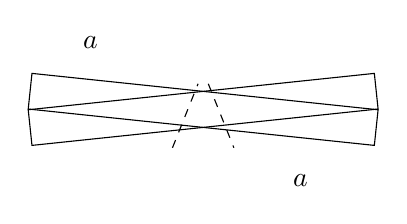
\begin{tikzpicture}[scale=0.65]
  % 图 15: 两个相交的长矩形
  \draw[rotate=6] (-3.4,-0.35) rectangle (3.4,0.35);
  \draw[rotate=-6] (-3.4,-0.35) rectangle (3.4,0.35);
  \draw[dashed] (-0.6,-0.75) -- (-0.1,0.5);
  \draw[dashed] (0.1,0.5) -- (0.6,-0.75);
  \node at (1.9,-1.4) {$a$};
  \node at (-2.2,1.3) {$a$};
\end{tikzpicture}
\caption{任意方向两相交矩形的重叠面积控制}
\label{fig:15}
\end{figure}

为控制这个交, 我们把它最大化: 在两个矩形确有相交的约束下, 平移诸 $\tilde{R}_{ij}$ 使二者之间的夹角最小.

我们还用最大的交来控制任何交; 即图~\ref{fig:15} 中所示的交. 按此做法, 这个交不随矩形左右滑动而变, 而由于列由 $i$ 编号, 我们所作的估计与 $i$ 无关. 于是为方便起见, 设 $i=i'$.

图~\ref{fig:15} 中交的面积容易计算; 每条虚线都是其中一个矩形的厚度, 即 $a$, 因为平行四边形的高为 $a$. 平行四边形的宽度满足 $\sin\theta=\frac{a}{N}$, 且
\[
\bigl|\tilde{R}_{i j}\cap\tilde{R}_{i' j'}\bigr|=\frac{a^{2}}{\sin\theta}
\]
(若 $\theta=0$, 这不准确; 修正将在下面给出).

给定条件 $\tilde{R}_{ij}\cap\tilde{R}_{i'j'}\neq\varnothing$ 与 $\tilde{R}_{ij}\cap Q_{i'j'}\neq\varnothing$, 角 $\theta$ 容易算出. 为使诸 $\tilde{R}_{ij}$ 的交最大, 角 $\theta$ 必须最小. 最小的 $\theta$ 出现在 $R_{ij}$ 与 $R_{i'j'}$ 恰好相触时, 如图~\ref{fig:16}.

\begin{figure}[htbp]
\centering
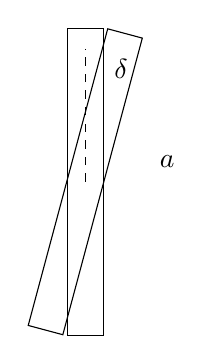
\begin{tikzpicture}[scale=0.65]
  % 图 16: 恰好相触的两个矩形
  \draw[rotate=90] (-3,-0.35) rectangle (3,0.35);
  \draw[rotate=75] (-3,-0.35) rectangle (3,0.35);
  \draw[dashed] (0,0) -- (0,2.6);
  \node at (0.7,2.2) {$\delta$};
  \node at (1.6,0.4) {$a$};
\end{tikzpicture}
\caption{临界相切矩形的夹角与边长关系}
\label{fig:16}
\end{figure}

则
\[
\sin\theta=\cos\Bigl(\frac{\pi}{2}-\theta\Bigr)\approx\frac{a\,|j-j'|}{\delta N}=\frac{|j-j'|}{N}.
\]
于是
\[
\bigl|\tilde{R}_{i j}\cap\tilde{R}_{i' j'}\bigr|\leq\frac{a^{2}N}{|j-j'|}.
\]
若 $j=j'$, 我们可以得到更好的估计, 故一般地,
\[
\bigl|\tilde{R}_{i j}\cap\tilde{R}_{i' j'}\bigr|\leq\frac{a^{2}N}{|j-j'|+1}.
\]
\end{proof}

\begin{remark}\label{rem:8.7}
上面对 $\mathcal{C}$ 的估计是最佳的; 我们现在证明这一事实. 取 $a=1$; 令当 $|x|\leq N$ 时 $f(x)=(1+|x|)^{-1}$, 其余情形 $f=0$. 则 $\|f\|_2\approx(\log N)^{\frac{1}{2}}$. 为估计 $\mathcal{C}f$, 先设 $|x|\leq N$. 取 $R_x$ 以 $\frac{x}{|x|}$ 为长边方向, 并选取它使 $R_x$ 的短边包含 $x$. 则 $|R_x|^{-1}\int_{R_x}f$ 是径向的, 我们在 $x=(|x|,0)$ 处求值:
\[
\frac{1}{N}\int_{-1}^{1}\int_{|x|-N}^{|x|}\frac{1}{1+|y|}\,dy_{1}\,dy_{2}
\geq C N^{-1}\int_{0}^{|x|}\frac{1}{1+y_{1}}\,dy_{1}
\geq C N^{-1}\log|x|.
\]
于是 $\|\mathcal{C}f\|_2^2\geq CN^{-2}\int_0^N\log^2 r\,dr\approx C\log^2 N$.
\end{remark}

\section{C\'ordoba 乘子定理}
\label{sec:8.3}

\begin{notation}\label{not:8.8}
设 $\phi$ 是 $\mathbb{R}^1$ 上满足当 $|x|>1$ 时 $\phi(x)=0$ 的光滑函数. 在 $\mathbb{R}^2$ 上定义 $\phi_\delta$ 为
\[
\phi_{\delta}(\xi)=\phi\bigl(\delta^{-1}(|\xi|-1)\bigr).
\]
设 $S_{\delta}$ 表示以 $\phi_{\delta}$ 为乘子的算子.
\end{notation}

\begin{theorem}\label{thm:8.9}
\index{Cordoba 乘子定理 (C'ordoba multiplier theorem)|emph}
\[
{}_{4}\|S_{\delta}\|\leq C\,|\log\delta|^{\frac{1}{4}}.
\]
\end{theorem}

\begin{proof}
以往那些乘子定理 (比如 Marcinkiewicz 定理) 的套路提示: 我们需要把 $\phi_{\delta}$ 的各个小块隔离开, 然后用一个极大函数控制各小块, 再控制极大函数. 许多部件已经就位; 例如极大函数的控制. 我们从定义小块开始.

直观上, 我们把 $\phi_\delta$ 想成厚度为 $\delta$ 的环形区域的特征函数. 我们希望彼此隔离的小块是不同的方向. 定理~\ref{thm:8.1} 中的函数将完成隔离, 但它不会把我们从 $S_\delta f$ 带到 $\bigl(\sum|S_jS_\delta f|^2\bigr)^{1/2}$; 相反, 它把我们从 $\sum|S_jf|^2$ 带到 $f$. 这意味着我们得自己做方向的隔离.

我们在~\ref*{ess:8.4} 中所做的计算提示, 若选取大小为 $\delta\times\delta^{\frac{1}{2}}$ 的矩形, 圆的曲率将提供隔离. 我们需要光滑地做这个分解; 取 $S^1$ 上的光滑函数 $\phi$, 设当 $|\theta|>\frac{1}{2}$ 时 $\phi(\theta)=0$, 并令
\[
\phi_{j}(\theta)=\phi\Bigl(\delta^{-\frac{1}{2}}\bigl(\theta-2\pi j[\delta^{\frac{1}{2}}]\bigr)\Bigr).
\]
我们再定义 $\mu_j(\xi)=\mu_j(r,\theta)=\phi_j(\theta)\,\phi_\delta(r)$, 并令 $T_j$ 表示相应的算子. 直观上, $\mu_j$ 是以 $j[\delta^{\frac{1}{2}}]$ 为中心、大小为 $\delta\times\delta^{\frac{1}{2}}$ 的矩形的特征函数. 如同~\ref*{ess:8.4} 中的讨论, 为避免不同方向之间的干扰, 我们需要把角度限制在圆的若干弧段上; 这相当于把所有最终估计乘一个因子 $8$. 于是我们可以假设 $0\leq j\leq[\delta^{-\frac{1}{2}}]/8$. 这些是我们的第一组分解.

开始估计:
\begin{align*}
\|S_{\delta}f\|_{4}^{4}
&=\Bigl\|\sum T_{j}f\Bigr\|_{4}^{4}
=\int\Bigl|\Bigl(\sum T_{j}f\Bigr)^{2}\Bigr|^{2} \\
&=\int\Bigl|\sum T_{j}f\,\sum T_{k}f\Bigr|^{2}
=\int\Bigl|\sum_{j,k}\widehat{T_{j}f}\star\widehat{T_{k}f}\Bigr|^{2}.
\end{align*}
由于每个 $x\in\mathbb{R}^2$ 至多属于 $9$ 个的 $\widehat{T}_jf\star\widehat{T}_kf=\mu_j\hat{f}\star\mu_k\hat{f}$ 的支集, 且这与 $\delta$ 无关, 最后的积分被
\begin{align*}
C\int\sum_{j,k}\bigl|\widehat{T_{j} f}\star\widehat{T_{k} f}\bigr|^{2}
&=C\int\sum_{j,k}|T_{j}f\,T_{k}f|^{2}
=C\int\sum_{j,k}|T_{j}f|^{2}\,|T_{k}f|^{2} \\
&=C\int\Bigl(\sum|T_{j}f|^{2}\Bigr)^{2}
=C\Bigl\|\Bigl(\sum|T_{j}f|^{2}\Bigr)^{\frac{1}{2}}\Bigr\|_{4}^{4}
\end{align*}
控制. 我们得到第一个分解:
\[
\|S_{\delta}f\|_{4}\leq C\Bigl\|\Bigl(\sum|T_{j}f|^{2}\Bigr)^{\frac{1}{2}}\Bigr\|_{4}.
\]
现在的任务是借助 $g$-函数从 $\sum|T_jf|^2$ 回到 $f$. 若令 $I_j$ 表示 $\phi_j$ 的支集在 $\xi_2$ 轴上的投影, 我们当然有 $\chi_{I_j}\mu_j=\mu_j$. 但注~\ref{rem:8.3} 对容许的 $I_j$ 提出了一些要求: 它们必须互不相交, 长度上下有界, 且彼此之间的距离有下界. 就目前而言, 我们取的 $\phi_j$ 是光滑的, 所以诸 $I_j$ 相互重叠. 这很容易克服: 把奇数与偶数的块分开处理, 把所有最终估计乘以 $2$. 我们甚至懒得改变记号. 于是诸 $I_j$ 互不相交, 长度为 $C\delta^{\frac{1}{2}}\sin(\frac{\pi}{2}-\theta_j)$, 其中 $\theta_j=2\pi j\delta^{\frac{1}{2}}$. 由于我们聪明地把 $0\leq\theta_j\leq\frac{\pi}{4}$ 限定了, 长度都被 $C\delta^{\frac{1}{2}}$ 控制. 当然, 诸 $I_j$ 之间的间距与缺失的块可比, 后者又与 $C\delta^{\frac{1}{2}}$ 可比. 于是我们可以用~\ref*{cor:8.2} 得到估计
\[
\Bigl\|\Bigl(\sum|S_{j}f|^{2}\Bigr)^{\frac{1}{2}}\Bigr\|_{4}\leq C\|f\|_{4},
\]
如果我们能走到那一步的话.

下一步是用极大函数控制 $T_jf$. 现在 $T_jf=\check{\mu}_j\star f$, 直观上 $\check{\mu}_j\star f$ 恰是在大小为 $\delta^{-1}\times\delta^{-\frac{1}{2}}$ 的矩形上对 $f$ 作平均. 设该矩形记为 $R_j$. 则 $T_jf\approx\frac{1}{|R_j|}\int_{R_j}f$, 且
\begin{align*}
\int|T_{j}f|^{2}\,g
&=\int\left|\int|R_{j}|^{-1}\chi_{R_{j}}(x-y)\,f(y)\,dy\right|^{2}g(x)\,dx \\
&\leq\int\left(\int\chi_{R_{j}}^{2}(x-y)\,dy\right)
\left(|R_{j}|^{-2}\int\chi_{R_{j}}^{2}(x-y)\,|f(y)|^{2}\,dy\right)g(x)\,dx \\
&=\int|R_{j}|\,|R_{j}|^{-2}\iint\chi_{R_{j}}(x-y)\,g(x)\,|f(y)|^{2}\,dy\,dx \\
&=\int|f(y)|^{2}\,|R_{j}|^{-1}\,\chi_{R_{j}}\star g\,dy.
\end{align*}
因此,
\[
\int\sum|T_{j}f|^{2}\,g=\int\sum|T_{j}S_{j}f|^{2}\,g
\leq\sum_j\int|S_{j}f|^{2}\,|R_{j}|^{-1}\chi_{R_{j}}\star g.
\]
若要沿 Marcinkiewicz 定理的证明走, 我们必须使 $|R_j|^{-1}\chi_{R_j}\star g$ 与 $j$ 无关. 我们对所有的 $j$ 取上确界来做到这一点; 这被一个对所有方向、大小为 $\delta^{-1}\times\delta^{-\frac{1}{2}}$ 的矩形所取的上确界控制. 这是一个 C\'ordoba 极大函数, 其中 $a=\delta^{-\frac{1}{2}}$, $N=\delta^{-\frac{1}{2}}$. 于是
\begin{align*}
\int\sum|T_{j}f|^{2}\,g
&\leq\int\sum|S_{j}f|^{2}\,\mathcal{C}(g) \\
&\leq\left(\int\Bigl(\sum|S_{j}f|^{2}\Bigr)^{2}\right)^{\frac{1}{2}}\|\mathcal{C}g\|_{2} \\
&\leq\Bigl\|\Bigl(\sum|S_{j}f|^{2}\Bigr)^{\frac{1}{2}}\Bigr\|_{4}^{2}\,\|\mathcal{C}g\|_{2} \\
&\leq C\|f\|_{4}^{2}\,\bigl(\log\delta^{-\frac{1}{2}}\bigr)^{\frac{1}{2}}\,\|g\|_{2}.
\end{align*}
对所有满足 $\|g\|_2=1$ 的 $g$ 取上确界:
\[
\Bigl\|\Bigl(\sum|T_{j}f|^{2}\Bigr)^{\frac{1}{2}}\Bigr\|_{4}^{2}
\leq C\,|\log\delta|^{\frac{1}{2}}\,\|f\|_{4}^{2},
\]
这就证明了定理.

当然, 还有很多技术细节. 我们并非在与一个矩形的特征函数作卷积. 另一方面, 卷积核属于 $\mathcal{S}$, 所以我们可以用 Schwartz 函数的想法来估计它. 首先, 注意诸 $\mu_j$ 都是同一个函数的旋转, 于是我们可以就其中一个 (记为 $K_0$) 估计卷积核. 直观上,
\[
K_{0}(x_{1},x_{2})=\delta^{\frac{3}{2}}\,\check{\phi}\bigl(\delta x_{1},\,\delta^{\frac{1}{2}}x_{2}\bigr),
\]
利用 $\phi\in\mathcal{S}$ 的想法,
\[
|K_{0}(x_{1},x_{2})|\leq C\,\delta^{\frac{3}{2}}\,|\delta x_{1}|^{-p}\,|\delta^{\frac{1}{2}}x_{2}|^{-q}
\]
对所有的 $p,q\geq 0$ 成立. 这意味着 $K_0$ 衰减得如此之快, 以至于我们可以用矩形特征函数之和来控制它. 令
\[
R_{i}^{0}=\{(x_{1},x_{2}) \mid |x_{1}|<2^{i}\delta^{-1},\ |x_{2}|<2^{i}\delta^{-\frac{1}{2}}\};
\]
我们断言
\[
|K_{0}(x)|\leq C\sum_{i}2^{-i}\,|R_{i}^{0}|^{-1}\chi_{R_{i}^{0}}(x).
\]
为证之, 取 $x\in R_{k+1}$; 设 $x$ 不在 $R_k$ 中. 若 $|x_1|>2^k\delta^{-1}$,
\[
|K_{0}(x)|\leq C\,\delta^{\frac{3}{2}}\,|\delta x_{1}|^{-3}\,|\delta x_{2}|^{0}
\leq C\,\delta^{\frac{3}{2}}\,\bigl|\delta\,2^{k}\delta^{-1}\bigr|^{-3}
=C\,\delta^{\frac{3}{2}}\,2^{-3k},
\]
而
\[
\sum_i 2^{-i}\,|R_{i}^{0}|^{-1}\chi_{R_{i}^{0}}(x)
=\sum_{i\geq k+1}2^{-i}\,\delta^{\frac{3}{2}}\,2^{-2i}
\approx C\,\delta^{\frac{3}{2}}\,2^{-3k}.
\]
证明的其余部分与之前一样:
\[
|T_{j}S_{j}f|\leq\sum_i 2^{-i}\,\Bigl||R_{i}^{j}|^{-1}\chi_{R_{i}^{j}}\star S_{j}f\Bigr|,
\]
且
\[
\Bigl\|\Bigl(\sum_j|T_{j}S_{j}f|^{2}\Bigr)^{\frac{1}{2}}\Bigr\|_{4}
\leq\sum_i 2^{-i}\,\Bigl\|\Bigl(\sum_j\bigl(|R_{i}^{j}|^{-1}\chi_{R_{i}^{j}}\star S_{j}f\bigr)^{2}\Bigr)^{\frac{1}{2}}\Bigr\|_{4}.
\]
由于 $2^{-i}$ 本身就可求和, 只需证明该 $L^{4}$ 范数关于 $i$ 一致有界. 这可以完全照旧去做, 只是矩形 $R_{i}^{j}$ 的尺寸为 $2^{i}\delta^{-1}\times2^{i}\delta^{-\frac{1}{2}}$. 这意味着我们取 C\'ordoba 极大函数, 其中 $a=2^{i}\delta^{-\frac{1}{2}}$, $N=\delta^{-\frac{1}{2}}$. 我们得到的范数 $\log N$ 与 $i$ 无关.

至此证明终于完成, 只差一个技术细节: $\mu_0$ 并非真的是方块的伸缩 $\psi\bigl(\delta^{-1}\xi_1,\delta^{-\frac{1}{2}}\xi_2\bigr)$. 真正的伸缩是在 $(r,\theta)$ 方向上, 这与 Fourier 变换配合得并不好. 现在我们展示如何克服这个问题. 我们的直观估计基于这样一个原理: 矩形的 Fourier 变换还是矩形; 它的精确版本考察 Schwartz 函数的导数. 首先,
\[
|x_{1}K_{0}|\leq\|x_{1}K_{0}\|_{\infty}\leq C\,\|D_{\xi_{1}}\mu_{0}\|_{1}.
\]
我们将证明
\[
\|D_{\xi_{1}}\mu_{0}\|_{1}\leq C\,\delta^{\frac{1}{2}},
\]
由此得到
\[
|K_{0}(x_{1},x_{2})|\leq C\,\delta^{\frac{3}{2}}\,|\delta x_{1}|^{-1},
\]
这正是我们所需要的典型结果.

首先,
\begin{align*}
D_{\xi_{1}}\mu&=\frac{\partial r}{\partial\xi_{1}}\,\frac{\partial\mu}{\partial r}
+\frac{\partial\theta}{\partial\xi_{1}}\,\frac{\partial\mu}{\partial\theta} \\
&=\frac{\xi_{1}}{(\xi_{1}^{2}+\xi_{2}^{2})^{\frac{1}{2}}}\,
\frac{\partial}{\partial r}\phi_{\delta}(r)\,\phi(\theta)
-\frac{\xi_{2}}{(\xi_{1}^{2}+\xi_{2}^{2})^{\frac{1}{2}}}\,
\phi_{\delta}(r)\,\frac{\partial}{\partial\theta}\phi(\theta).
\end{align*}
对 $\xi\in\operatorname{support}\mu_0$, 有 $|\xi_1|\leq 2$, $\xi_1^2+\xi_2^2\geq\frac{1}{2}$, $|\xi_2|\leq 2$, 且当然有
\[
\frac{\partial\phi_{\delta}}{\partial r}=\delta^{-1}\phi'\bigl(\delta^{-1}(r-1)\bigr),
\qquad
\frac{\partial\phi}{\partial\theta}=\delta^{-\frac{1}{2}}\phi'\bigl(\delta^{-\frac{1}{2}}\theta\bigr).
\]
于是,
\[
|D_{\xi_{1}}\mu_{0}|\leq C\,\delta^{-1}\bigl(|\phi'\psi|+\delta^{\frac{1}{2}}\,|\phi\psi'|\bigr)
\leq C\,\delta^{-1}.
\]
最后,
\[
\|D_{\xi_{1}}\mu_{0}\|_{1}\leq C\,\delta^{-1}\,|\operatorname{support}\mu_{0}|
=C\,\delta^{-1}\,\delta^{\frac{3}{2}}.
\]
这个估计以及类似的估计完成了定理的证明.
\end{proof}

\begin{corollary}\label{cor:8.10}
Bochner--Riesz 平均在最优范围内有界.
\end{corollary}

\begin{proof}
我们从一个单位分解 $1=\sum_i\phi_i$ 出发. 设诸 $\phi$ 光滑、径向, 径向支在 $[1-2^{-i},\,1-2^{-i-2}]$ 中, 且 $|D_r^p\phi_i|\leq C2^{ip}$. 令 $\mu_i=\phi_i\mu_\lambda$; 注意 $\mu_\lambda=\sum_i\mu_i$.

直观上, $\mu_i$ 近似是 $\phi_i$ 乘以 $\mu_\lambda$ 在 $\phi_i$ 支集上的最大值, 即 $2^{-\lambda i}$. 因此 $\mu_i$ 的 $L^4$ 范数应当如同 $2^{-\lambda i}\,\bigl|\log 2^{-i}\bigr|^{\frac{1}{4}}$. 若 $\lambda>0$, 这可以对和求和, 于是只要 $\lambda>0$, 所有的 Bochner--Riesz 算子 $T_\lambda$ 都在 $L^4$ 上有界. 内插现在给出最优范围的其余部分.

当然这只是直观; 为给出精确的证明, 我们重新审视~\ref*{thm:8.9} 的证明. 我们注意到, 取 $\delta=2^{-i}$ 时, $\mu_i$ 具有那里用到的 $\phi_\delta$ 的一切性质. 在照搬那个证明之前, 唯一需要验证的是对 $|K_0|$ 的估计. 我们将证明
\[
|K_{0}(x_{1},x_{2})|\leq C\,\delta^{\lambda}\,\delta^{\frac{3}{2}}\,|x_{1}\delta|^{-p}\,|x_{2}\delta^{\frac{1}{2}}|^{-q},
\]
而如同~\ref*{thm:8.9}, 这给出 $L^4$ 范数 $\delta^{\lambda}\,|\log\delta|^{\frac{1}{4}}$, 这正是我们需要的.

对 $K_{0}$ 的估计遵循与~\ref*{thm:8.9} 中相同的模式. 一个典型的估计要求
\[
\left|\frac{\partial}{\partial r}\mu_{i}\right|\leq\delta^{\lambda}\,\delta^{-1}.
\]
但
\[
\left|\frac{\partial}{\partial r}\mu_{i}\right|
\leq\left|\frac{\partial}{\partial r}\phi_{i}\,\mu_{\lambda}\right|
+\left|\frac{\partial}{\partial r}\mu_{\lambda}\,\phi_{i}\right|.
\]
现在 $\bigl|\frac{\partial}{\partial r}\phi_i\bigr|\leq C2^i$, 而若 $r\in\operatorname{support}\phi_i$, 则 $\bigl|\mu_\lambda(r)\bigr|\leq\delta^\lambda$. 类似地,
\[
\left|\frac{\partial}{\partial r}\mu_{\lambda}\right|\leq C\,\bigl|(1-r^{2})^{\lambda-1}\bigr|,
\]
而对 $r\in\operatorname{support}\phi_i$, 有 $1-\delta<r<1-\frac{\delta}{4}$, 故
\[
\left|\frac{\partial}{\partial r}\mu_{\lambda}\right|\leq C\,\delta^{\lambda-1}.
\]
其余的估计照~\ref*{thm:8.9} 的证明进行.
\end{proof}

\section{重访限制性}
\label{sec:8.4}

在本节中, 我们将证明 $\mathbb{R}^2$ 中限制性在最优范围内的 $L^p$--$L^q$ 有界性. 我们从标准模型开始; 我们考察一个环形区域而非单位圆. 注意
\[
\int_{S^{1}}\bigl|\hat{f}(\theta)\bigr|^{q}\,d\theta
=\lim_{\delta\to0}\frac{1}{2\delta}\int_{1-\delta}^{1+\delta}\int_{S^{1}}\bigl|\hat{f}(r,\theta)\bigr|^{q}\,r\,dr\,d\theta,
\]
于是我们可以由环形区域恢复出限制性. 设 $0\leq\phi\leq 1$ 如~\ref*{not:8.8} 中那样, 且 $\chi_{(1-\delta,1+\delta)}(|\xi|)\leq\phi_\delta(\xi)$. 只需证明
\[
\frac{1}{2\delta}\int_{1-\delta}^{1+\delta}\int_{S^{1}}\bigl|\phi_{\delta}(r)\,\hat{f}(r,\theta)\bigr|^{q}\,r\,dr\,d\theta\leq C\|f\|_{p}^{q},
\]
亦即
\[
\bigl\|\phi_{\delta}\hat{f}\bigr\|_{L^{q}(S^{1})}\leq\delta^{\frac{1}{q}}\,\|f\|_{p}.
\]
设 $Rf=\phi_{\delta}\hat{f}$; 则
\[
R^{\star}g=\widehat{\phi_{\delta}\,g}=\check{\phi}_{\delta}\star g=S_{\delta}g.
\]

\begin{theorem}\label{thm:8.11}
\index{离散分数次积分 (discrete fractional integration)}
设 $q=\frac{p'}{3}$. 则
\begin{align*}
\|S_{\delta}g\|_{p'}&\leq C\,\delta^{\frac{1}{q}}\,\|g\|_{q'},\qquad 1\leq p<\frac{4}{3}, \\
\|S_{\delta}g\|_{4}&\leq C\,\delta^{\frac{3}{4}}\,|\log\delta|^{\frac{1}{4}}\,\|g\|_{4}.
\end{align*}
\end{theorem}

\begin{proof}
若 $p\leq\frac{4}{3}$, 则 $r=\frac{p'}{2}\geq 2$, 且
\begin{align*}
\|S_{\delta}g\|_{p'}^{p'}
&=\|S_{\delta}g\cdot S_{\delta}g\|_{r}^{r}
\leq\bigl\|\widehat{S_{\delta}g}\star\widehat{S_{\delta}g}\bigr\|_{r'}^{r}
=\|(\phi_{\delta}\check{g})\star(\phi_{\delta}\check{g})\|_{r'}^{r} \\
&=\Bigl\|\sum_{j,k}(\phi_{\delta}\phi_{j}\check{g})\star(\phi_{\delta}\phi_{k}\check{g})\Bigr\|_{r'}^{r} \\
&\leq C\left(\sum_{j,k}\int\bigl|(\phi_{\delta}\phi_{j}\check{g})\star(\phi_{\delta}\phi_{k}\check{g})\bigr|^{r'}\right)^{\frac{r}{r'}};
\end{align*}
最后一步用了~\ref*{thm:8.9} 证明中的殆正交性. 我们稍后将证明: 若 $1\leq r'\leq\infty$, 则
\[
\bigl\|(\phi_{\delta}\phi_{j}f)\star(\phi_{\delta}\phi_{k}f)\bigr\|_{r'}
\leq C\left[\frac{\delta^{\frac{3}{2}}}{|j-k|+1}\right]^{\frac{1}{r}}\|\phi_{j}f\|_{r'}\,\|\phi_{k}f\|_{r'}.
\]
这给我们一个界
\[
C\delta^{\frac{3}{2}}\left(\sum_{k}\|\phi_{k}f\|_{r'}^{r'}\left[\sum_{j}\frac{\|\phi_{j}f\|_{r'}^{r'}}{(|j-k|+1)^{\frac{r'}{r}}}\right]\right)^{\frac{r}{r'}}.
\]
令 $b_j=\|\phi_jf\|_{r'}^{r'}$. 则我们需要控制
\begin{align*}
&\,C\delta^{\frac{3}{2}}\left(\sum_{k}b_{k}\left[\sum_{j}\frac{b_{j}}{(|j-k|+1)^{\frac{r'}{r}}}\right]\right)^{\frac{r}{r'}} \\
&\leq C\delta^{\frac{3}{2}}\left(\sum_{k}b_{k}^{s}\right)^{\frac{r}{r's}} \\
&\qquad\times\left(\sum_{k}\left[\sum_{j}b_{j}\,(|j-k|+1)^{1-r'}\right]^{s'}\right)^{\frac{r}{r's'}}.
\end{align*}
若 $p<\frac{4}{3}$, 则 $2-r'>0$, 我们选取 $\frac{1}{s'}=\frac{1}{2}-(2-r')$, 并用离散分数次积分理论 (Hardy--Littlewood--P\'olya~\cite{hardy-littlewood-polya}) 得到界
\[
C\delta^{\frac{3}{2}}\left(\sum_{k}b_{k}^{s}\right)^{\frac{2r}{r's}}.
\]
但 $r's=q'$, 于是我们可以用 H\"older 不等式从 $r'$ 过渡到 $q'$ 来估计 $\|\phi_jf\|_{r'}^{r'}$. 这给出
\begin{align*}
C\delta^{\frac{3}{2}}\,\delta^{\frac{3}{2}\left(\frac{q'}{r'}-1\right)\frac{2r}{q'}}\left(\sum_{k}\int|\phi_{k}f|^{q'}\right)^{\frac{2r}{q'}}
&=C\delta^{3}\,\|f\|_{q'}^{2r}.
\end{align*}
这正是我们需要的.

另一方面, 若 $p=\frac{4}{3}$, 则 $r'=r=s=s'=2$, 于是我们可以用估计
\[
\left(\sum_{k}\left[\sum_{j}\frac{b_{j}}{|j-k|+1}\right]^{2}\right)^{\frac{1}{2}}
\leq\left(\sum_{k}(|j-k|+1)^{-1}\right)\left(\sum_{j}b_{j}^{2}\right)^{\frac{1}{2}}.
\]
这给我们一个界
\begin{align*}
C\delta^{\frac{3}{2}}\,|\log\delta|\,\sum_{j}b_{j}^{2}
&=C\delta^{\frac{3}{2}}\,|\log\delta|\sum_{j}\|\phi_{j}f\|_{2}^{4}
\leq C\delta^{\frac{3}{2}}\,|\log\delta|\,\|f\|_{4}^{4}.
\end{align*}
为证明估计
\[
\bigl\|(\phi_{\delta}\phi_{j}f)\star(\phi_{\delta}\phi_{k}f)\bigr\|_{r'}
\leq C\left[\frac{\delta^{\frac{3}{2}}}{|j-k|+1}\right]^{\frac{1}{r}}\|\phi_{j}f\|_{r'}\,\|\phi_{k}f\|_{r'},
\]
我们使用双线性内插. 若 $B(f,g)=f\star g$ 是双线性映射
\[
B:L^{p}(S_{j})\times L^{p}(S_{k})\to L^{p}(S_{j}+S_{k}),
\]
我们将从 $p=1$ 与 $p=\infty$ 对 $B$ 作内插. 则
\begin{align*}
\|(\phi_{\delta}\phi_{j}f)\star(\phi_{\delta}\phi_{k}f)\|_{1}
&\leq\|\phi_{\delta}\phi_{j}f\|_{1}\,\|\phi_{\delta}\phi_{k}f\|_{1} \\
&\leq\|\phi_{\delta}\|_{\infty}^{2}\,\|\phi_{j}f\|_{1}\,\|\phi_{k}f\|_{1}
=\|\phi_{j}f\|_{1}\,\|\phi_{k}f\|_{1}.
\end{align*}
在 $p=\infty$ 的情形,
\[
\|(\phi_{\delta}\phi_{j}f)\star(\phi_{\delta}\phi_{k}f)\|_{\infty}
\leq\|\phi_{\delta}\|_{\infty}^{2}\,\|\phi_{j}f\|_{\infty}\,\|\phi_{k}f\|_{\infty}\,\|\phi_{j}\star\phi_{k}\|_{\infty}.
\]
惯常的``平行四边形面积''技巧给出
\[
\|\phi_{j}\star\phi_{k}\|_{\infty}\leq C\,\frac{\delta^{\frac{3}{2}}}{|j-k|+1},
\]
于是内插证明了结果.
\end{proof}

\begin{remark}\label{rem:8.12}
\begin{enumerate}[label=\alph*)]
\item 已经知道限制性定理在 $p=\frac{4}{3}$ 处失效; 因子 $|\log\delta|$ 的出现解释了这一失效.
\item 容易证明这个估计是最优的; 设 $S_j=\operatorname{support}\phi_j$, 并令 $g\equiv 1$. 则 $\|g\|_4^4=\delta$, 且
\[
\|S_{\delta}\hat{g}\|_{4}^{4}=\int\Bigl|\sum_{j,k}\chi_{S_{j}}\star\chi_{S_{k}}\Bigr|^{2}
\geq\sum_{j,k}\int\bigl|\chi_{S_{j}}\star\chi_{S_{k}}\bigr|^{2}.
\]
但 $\chi_{S_{j}}\star\chi_{S_{k}}\geq C\frac{\delta^{\frac{3}{2}}}{|j-k|+1}$ 在 $\chi_{S_{j}}\star\chi_{S_{k}}$ 的支集的至少一半上成立, 而后者的测度至少为 $C\delta^{\frac{3}{2}}(|j-k|+1)$. 于是
\[
\|S_{\delta}\hat{g}\|_{4}^{4}
\geq C\delta^{3}\,\delta^{\frac{3}{2}}\sum_{j,k}\bigl(|j-k|+1\bigr)^{-1}
=C\delta^{3}\,\delta^{\frac{3}{2}}\,\delta^{-\frac{1}{2}}\,|\log\delta|.
\]
\item 这些计算与我们``除非 $\widehat{d\sigma}\in L^p$, 否则限制性必失效''的直观有关. 如上, 令 $\hat{g}\equiv 1$; 则 $S_{\delta}\hat{g}=\hat{\phi}_{\delta}$, 且上面的估计表明
\[
\|\hat{\phi}_{\delta}\|_{4}\approx C\,\delta^{\frac{3}{4}}\,|\log\delta|^{\frac{1}{4}},
\]
而这个估计是最优的. 由于 $d\sigma=\lim_{\delta\to0}\delta^{-1}\phi_{\delta}$, 我们再次看到 $\widehat{d\sigma}$ 不属于 $L^4$. 这也可以与曲率性质联系起来; 我们需要知道没有一个 $\xi$ 落在多于 $9$ 个的 $S_j+S_k$ 之中, 而且
\[
\bigl|\chi_{S_{j}}\star\chi_{S_{k}}\bigr|\leq\frac{|S_{j}|}{|j-k|+1}.
\]
这两个性质对直线来说都惨遭失败. 例如, 设 $S=[-1,1]\times\{0\}$, $D_j=\bigl[j\delta^{\frac{1}{2}},(j+1)\delta^{\frac{1}{2}}\bigr]\times[-\delta,\delta]$, $-\delta^{-\frac{1}{2}}\leq j\leq\delta^{-\frac{1}{2}}$. 则原点落在所有的 $D_j+D_k$ 之中, 于是重叠是巨大的. 类似地, $\|\chi_{D_j}\star\chi_{D_k}\|_{\infty}=|D_j|$, 于是我们得不到任何随 $j-k$ 的衰减.
\end{enumerate}
\end{remark}

\section{评注与推广}
\label{sec:8.5}

\noindent (定理~\ref{thm:8.1}):\quad 这个结果取自 C\'ordoba~\cite{cordoba-kakeya}, 不过 C\'ordoba 说明它更早便已为人所知. 最近有人证明, 对间距与一致性的要求可以完全去掉; 结果对任意互不相交的区间都成立.

\noindent (注~\ref*{ess:8.4}):\quad 殆正交性最早出现在 C.~Fefferman~\cite{fefferman-spherical} 中; 一个较弱的版本被用于 C.~Fefferman 与 E.~M.~Stein~\cite{fefferman-stronglysingular} 的一个限制性定理. 在后者中, 人们用到这样一个事实: 每个长度与方向恰好对应圆上至多两条弦. $S_{j}+S_{k}$ 中的一个点对应于稍微加厚的圆上的一个方向与一个长度.

\noindent (定理~\ref{thm:8.6}):\quad 这里的证明取自 C\'ordoba~\cite{cordoba-kakeya}. 通过伴随控制极大函数的想法最早由 C\'ordoba 发展; 参见~\cite{deguzman} 的附录. 原始想法可追溯到 Kolmogorov--Seliverstov--Plessner 定理; 参见 Zygmund~\cite{zygmund}.

关于这些极大函数有界性的其他证明, 见 Wainger~\cite{wainger-applications}.

\noindent (定理~\ref{thm:8.9}):\quad 这里的证明取自 C\'ordoba~\cite{cordoba-bochnerriesz}. 对 $T_{\delta}$ 的控制最早由 C\'ordoba~\cite{cordoba-kakeya} 建立, 不过在那种情形必须先控制一个强得多的极大函数, 即``Kakeya 极大函数''. 它取遍所有边长之比为 $N$ 的矩形上的平均. 这些想法可以追溯到 C.~Fefferman 的文章~\cite{fefferman-spherical}.

\noindent (推论~\ref{cor:8.10}):\quad 这个结果最早由 L.~Carleson 与 P.~Sj\"olin~\cite{christ} 证明. 证明的途径是把卷积核分解成小块, 如同~\ref*{thm:6.9} 中那样; 然后以直接的方式遵循~\ref*{sec:6.1} 中的直观. Carleson 与 Sj\"olin 不是证明 $T_{\lambda}$ 的各部分如同限制算子, 而是先证明 Plancherel 型的估计, 再证明 $L^{4}$ 型的估计.

~\ref*{cor:8.10} 的第二个证明由 C.~Fefferman~\cite{fefferman-spherical} 给出; 从历史上看, 它出现在 Kakeya 集被引进之后, 并且是第一篇把 Kakeya 集思想融入正面结果的论文.

\noindent (定理~\ref{thm:8.11}):\quad 当 $p\neq\frac{4}{3}$ 时这个结果的第一个证明归功于 C.~Fefferman 与 E.~M.~Stein~\cite{fefferman-spherical}; C\'ordoba~\cite{cordoba-flp} 给出了一个几何证明. 由环形区域出发的结果是~\cite{tomas2} 中证明的简化版本.
